
%
\section{Identity by descent}
%

Relatedness among individuals is a natural property of genetic inheritance.
Although this observation may seem trivial as we all inherit our DNA from somebody,\footnote{Until CRISPR/Cas9 genome editing has been established \citep[\eg see][]{Cai:2016km}; in reference to the term \emph{\glsentrylong{ibd}}~(IBD) I propose the term \emph{identity by modification}, or IBM. {\color{oxgray}[\textit{Castigat ridendo mores}]}} knowledge about the genetic relationship between individuals is crucial to many applications in genetic research.
The validation of individual relationships is of particular interest in family-based methods such as linkage analysis \citep{Purcell:2007dg,Albrechtsen:2009cb}, or to exclude pedigree errors that would influence statistical power in linkage studies \citep{Boehnke:1997ku}, but also in population-based (case-control) association studies of purportedly unrelated individuals, where unreported relatedness may lead to spurious results due to population stratification, \ie systematic differences in the ancestry of individuals \citep{Freedman:2004dk,Voight:2005cr}.

The relationship between individuals is indicated by the alleles they have in common, where \n{2} alleles are said to be \emph{identical by descent} if they have been co-inherited from a common ancestor \citep{Thompson:1974fi,Thompson:1975uu}.
The concept of \glsentryfull{ibd} was introduced by \citet{cotterman1940calculus} and extended by \citet{malecot1948mathematics} who provided probability formulations of IBD in related individuals; the term ``identity by descent'' was coined by \citet{crow1954}.
Notably, \citet{malecot1948mathematics} defined IBD as the probability that no mutation occurred since the common ancestor; see also \citet{Slatkin:2008by}.
In contrast, \gls{ibs} refers to alleles that are observed to be the ``same'', but which may not be shared by descent.

Traditional measures of relatedness define IBD as the gametic relationship at a single locus, for which in particular the inbreeding coefficient and the kinship coefficient introduced by \citet{Wright:1921tk,Wright:1922cr} have been relevant.
For example, the probability that \n{2} homologous alleles are identical by descent in the same diploid individual is given by the inbreeding coefficient.
However, such traditional approaches often assume that the relationship status of the individuals is known or can be derived from possible pedigree relationships, where ancestors are defined with respect to the founders of a pedigree.
It has been argued that ancestry defined in reference to a founder sample is ``something arbitrary'' \citep[][p~141]{maynardsmith1989}; see \citet{Rousset:2002bz}.
Moreover, this definition of IBD (in particular the distinction between IBD and IBS) seems to be in conflict with coalescent theory, which postulates that every allele is technically identical by descent in the individuals which carry them, because all shared mutations in the genome can be traced back to a common ancestor at different times in the past \citep{Powell:2010di}.

Given the recent advances in genotyping and sequencing technologies, single-locus concepts of IBD have become less common and are supplanted by genealogically defined concepts of \emph{haplotype sharing by decent} in large samples of unrelated individuals \citep{Thompson:2013cj,Wakeley2016book}.
For example, the inference of IBD sharing has been useful to provide information about historical migration events and to reconstruct the demographic history of a population \citep{Palamara:2012cya,Palamara:2013eg,Harris:2013id}.
If an allele at a given locus has recently been co-inherited \n{2} or more individuals, it is likely that alleles at the surrounding loci on the same chromosome were also derived from the same ancestral lineage in those individuals, due to genetic linkage through the process of meiotic recombination.
The definition of IBD is therefore extended to refer to \n{2} homologous chromosomal \emph{segments} that are identical by descent if they have been co-inherited without intervening recombination from a common ancestor \citep{Hayes:2003gj,Powell:2010di}, such that the genealogical relationship between \n{2} haplotypes is the same along the shared region.
Consequently, meiotic recombination is seen as the driving force that shapes the patterns of relatedness among individuals.
Note that this definition regards relatedness as the pairwise relationship between \n{2} gametes, as any pair of chromosomes
The length of a shared IBD segment is delimited by the rate of recombination in each generation.
Note that IBD denotes a pairwise relationship between chromosomes as

Note that recombination events may not always result in the termination of an IBD segment.
This is because a coalescent event may join the \n{2} lineages broken up by recombination back together (back in time), forming a `closed loop' in the \gls{arg} \citep[see][Theorem~2.4]{griffiths1997ancestral}.


-- Recent advances in high-throughput sequencing technologies; thus not having pedigree information and no reference to a founder

-- However, this definition of IBD stands in contrast to insights from coalescent theory in which all alleles can be traced back to a common ancestor albeit at different times in the past; except for private mutations (de novo) or recurrent mutations



-- Each individual has $2^t$ ancestors at $t$~generations ago;
-- Theoretical considerations suggest that ancestors further back than a few generations do not contribute genetic material to our genome {Donnelly:1983fi}



Traditionally, relatedness has been quantified based on coefficients of relationship \citep{Wright:1921tk,Wright:1922cr}, in particular the kinship coefficient and inbreeding coefficient.


% One of the key features of genetic variation,

% Concepts of relatedness, measuring the genetic relation- ships among individuals, are basic to population genetics. They were initially conceived as measures of genetic likeness due to recent shared ancestry given by pedigree relationships, and as such they are standard tools in quantitative genetics and in kin selection theory.

% The concept of identity by descent (IBD) was classically quantified1 following Wright’s work on the coefficients of relationship2,3 and is used to indicate two homologous alleles that have descended from a common ancestor. This fundamental concept has many uses in genetics, including predicting genotype frequencies4, mapping genes5,6, estimating genetic variance7 and predicting inbreeding depression8.


%all individuals are related if traced back far enough and some pairs of individuals are more closely related than others despite all being called ‘unrelated’.

%that all chromosomes ultimately share a common ancestor


if they have co-inherited this segment from a common ancestor
such that
these individuals share the same ancestral origin

concept of IBD
haplotype sharing by decent
If an allele at a given locus is identical by descent in \n{2} or more individuals, it is likely that the surrounding loci nearby on the same chromosome were derived from the same ancestral lineage in those individuals.



genetic similarity
differences of allelic states along the haplotype region


For example,
\citep{Chapman:2003jt}


%
%!TEX root = ../../main.tex


\begin{figure}[p]
{\small\texthv{\textbf{(a)}}} \\
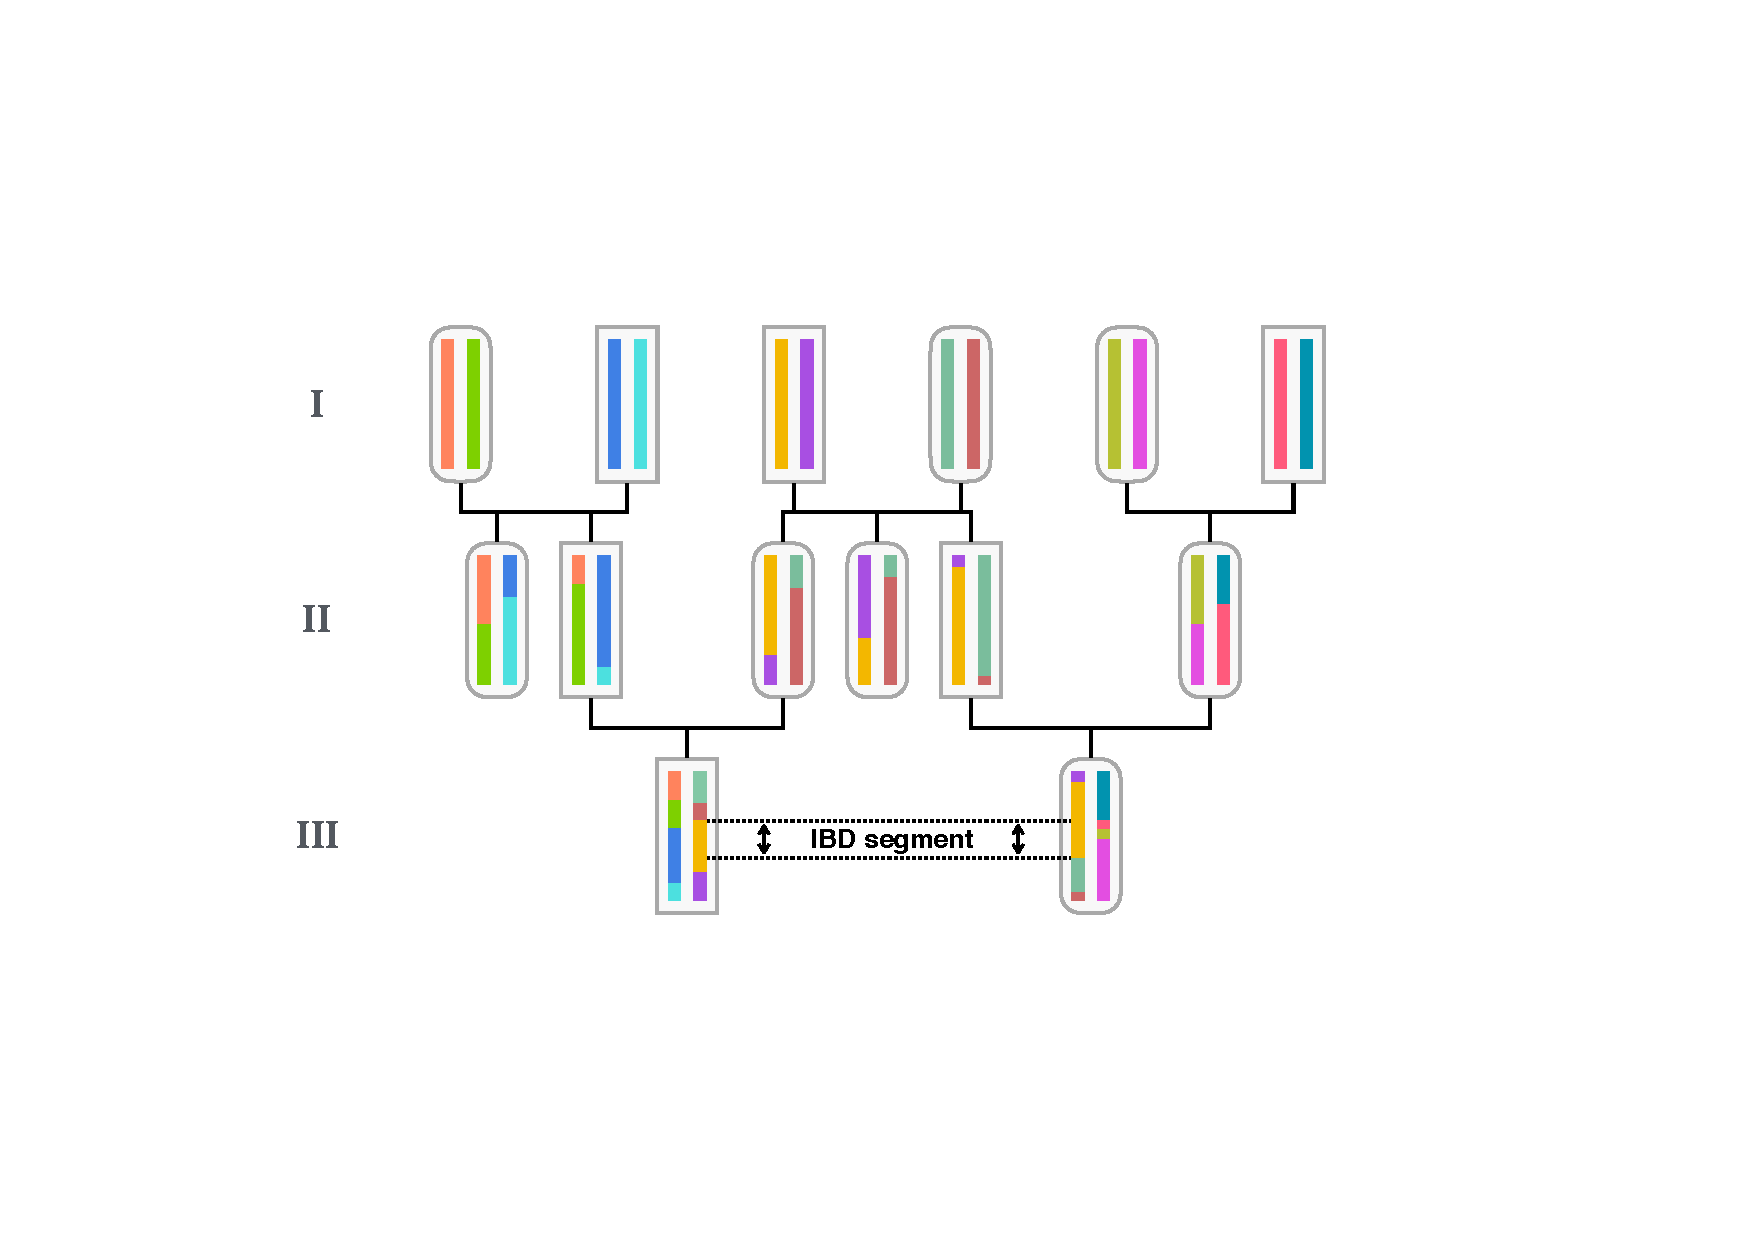
\includegraphics[width=\textwidth]{./img/ch1/info_ibd}
{\small\texthv{\textbf{(b)}}} \\
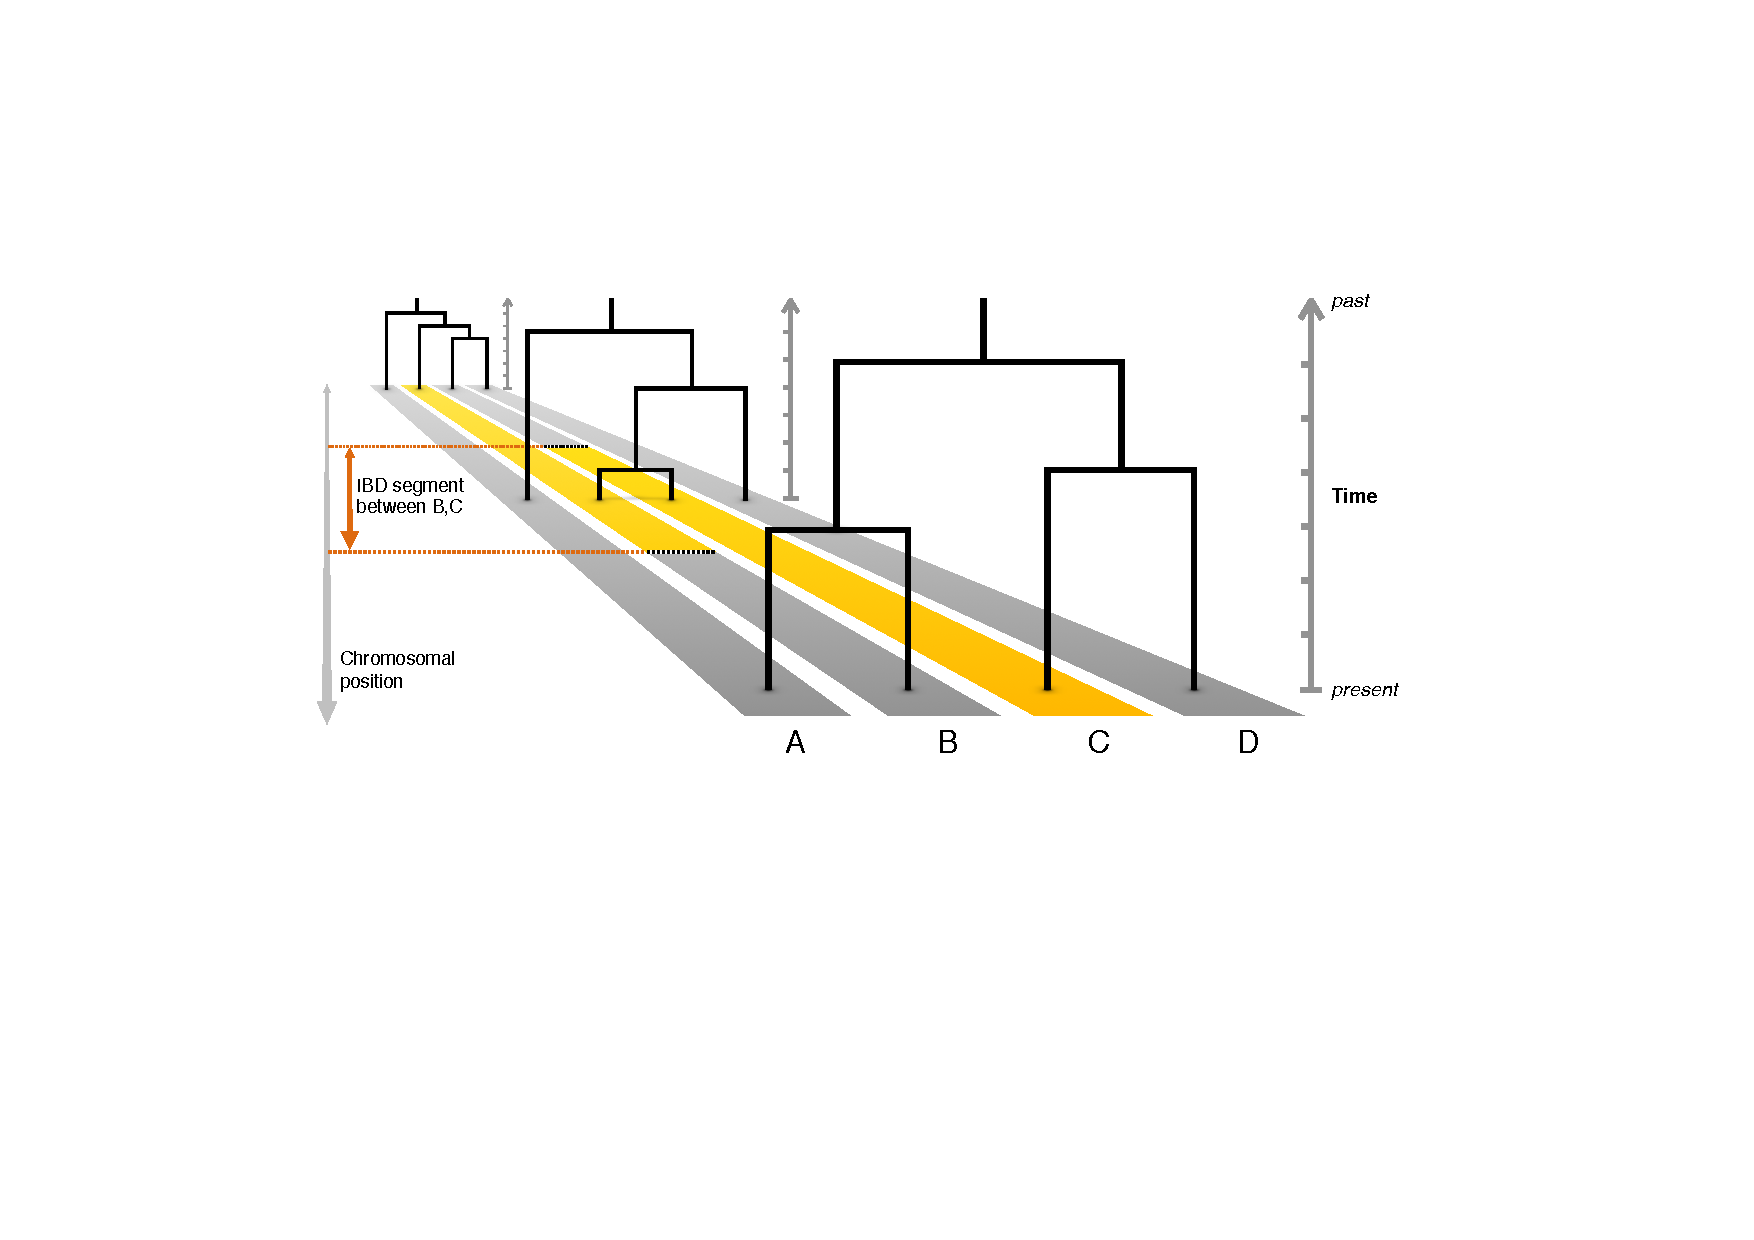
\includegraphics[width=\textwidth]{./img/ch1/info_ibd_segment}
\Caption{Illustration of haplotype sharing by descent}
{Panel~\textbf{(a)} shows a \n{3}-generation pedigree; generation~\rom{1} consists of the founders of the pedigree.
The \n{2} individuals shown in generation~\rom{3} are first-degree cousins.
Male and female individuals are distinguished by square and round shapes, respectively.
Each individual carries a diploid genome, shown as \n{2} large homologous chromosomes.
The colour of each chromosome indicates the ``identity'' of the shared ancestral haplotype, which is shuffled with the other haplotype present in the same individual due to meiotic recombination in each generation, such that the offspring receives a unique arrangement of haplotype segments per chromosome from each parent.
The ``shared'' haplotype refers the the overlapping region of haplotypes that are identical by descent; \ie the IBD segment shared by the \n{2} individuals in generation~\rom{3}, indicated by the \emph{orange} ancestral haplotype.
For simplicity, all founders are shown with the same colour.
Panel~\textbf{(b)} illustrates the different genealogies along the length of the sequence of \n{4} chromosomes (A, B, C, and D), indicated by \n{3} marginal trees.
The IBD segment co-inherited by chromosomes B and C is found at the overlapping region of the shared ancestral haplotype of the \gls{mrca} (\emph{orange}).
Note that the \n{4} chromosomes given in Panel~(b) show a simpler arrangement of haplotypes than shown in Panel~(a).}
{fig:info_ibd}
\end{figure}

%




recently inherited IBD (\eg $<100$ generations) \citep{Browning:2008es}.



-- Importantly, haplotype sharing by descent may not imply that the allelic sequence along the shared region is identical in both chromosome.




% IBD detection methods are often haplotype-based requiring the statistical
% estimation of haplotypes prior to analysis. The presence of phasing errors significantly
% decreases power to detect IBD segments (Browning and Browning [2012],
% Palamara and Pe'er [2013]). Power is critically linked to genotyping errors as well
% (Browning and Browning [2012]), and therefore stringent data quality control is
% essential even for methods that allow some discordance to exist within shared
% IBD chunks.
